\documentclass{standalone}
\usepackage[T1]{fontenc}
\usepackage[utf8]{inputenc}
\usepackage{pgf,tikz}
\usepackage{setspace}
\usepackage{pgfplots}
\pgfplotsset{compat=1.13}
\usepgfplotslibrary{fillbetween}

\begin{document}

\def\sysCont{2*tf([1], [1, 0])*tf([2], [1, 2])*tf([3], [1, 3]);}
\def\samplePeriod{0.3}


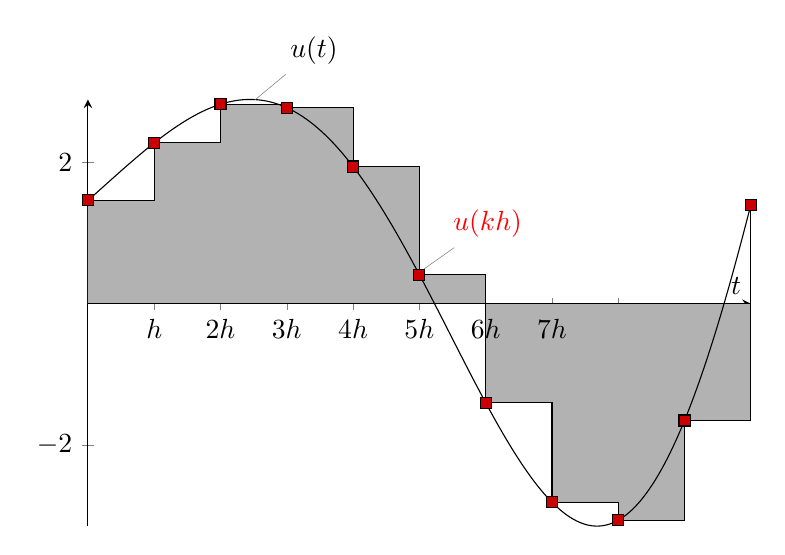
\begin{tikzpicture}
  \begin{axis} [
    clip=false,
    width=10cm,
    height=7cm,
    axis lines=middle,
    xlabel={$t$},
    xtick={1,2,3,4,5,6,7,8},
    xticklabels={$h$, $2h$, $3h$, $4h$, $5h$, $6h$, $7h$},
    ]
    \addplot+ [black, no marks, domain=0:10, samples=400] {exp(0.15*(x+2))*sin(deg(0.6*x)+20) + 1} node[coordinate, pos=0.18, pin=45:{$u(t)$}] {};
    %\addplot+ [name path=A, red, ycomb, domain=0:10, samples=11] {exp(0.15*(x+2))*sin(deg(0.6*x)+20) + 1} node[coordinate, pos=0.4, pin=45:{$u(kh)$}] {};
    \addplot+ [name path=A, const plot, red, draw=black,  domain=0:10, samples=11] { (x>-1)* (exp(0.15*(x+2))*sin(deg(0.6*x)+20) + 1)} node[coordinate, pos=0.4, pin=45:{$u(kh)$}] {};
    \addplot+ [name path=B, black, no marks, domain=0:10, samples=2] {0};

    \addplot[black!30] fill between[of=A and B];
  \end{axis}
  
\end{tikzpicture}

\end{document}
